\newpage
\section{DESARROLLO Y ANÁLISIS DE RESULTADOS}

A continuación se muestran los métodos de desarrollo utilizados para resolver cada uno de los problemas planteados, así como la funciones utilizadas, el método de operación a partir de diagramas de flujo y los resultados obtenidos:

\subsection{Desarrollo de la solución}

A continuación podrá consultarse una descripción de alto nivel de cada una de las funciones implementadas en el código .ino generado por Edge Impulse que contiene el modelo entrenado y optimizado. Además se incluye la descripción del código relacionado con el control del RGB, agregado al primero:

\subsubsection{Función \texttt{OV7675::begin()}}
Esta función inicializa la cámara OV7675 con los parámetros especificados de resolución, formato y velocidad de fotogramas. La cámara debe ser configurada correctamente para asegurar que los datos de imagen capturados sean coherentes con los requisitos de la aplicación.

\subsubsection{Función \texttt{OV7675::readFrame()}}
Esta función es responsable de leer un fotograma desde la cámara OV7675 y almacenarlo en el búfer proporcionado como argumento. Esto implica la transferencia de datos desde el sensor de la cámara a la memoria del microcontrolador o procesador.

\subsubsection{Función \texttt{setup()}}
La función setup es parte del ciclo de vida básico de un programa Arduino. En este contexto, configura el entorno inicial del programa, establece la comunicación serial y proporciona información sobre la configuración actual de la inferencia de Edge Impulse. Esto incluye la configuración de pines, inicialización de periféricos y otros ajustes necesarios antes de la ejecución principal del programa.

\subsubsection{Función \texttt{loop()}}
La función loop se ejecuta de forma repetitiva después de setup. En este caso específico, gestiona la captura de imagen, el procesamiento y la inferencia utilizando Edge Impulse. Controla la lógica de inicio y parada de la inferencia basada en la entrada del usuario o condiciones predefinidas.

\subsubsection{Función \texttt{ei\_camera\_init()}}
Es una función que inicializa la cámara para su uso. Esto podría incluir la configuración de los registros de la cámara para establecer la resolución, el formato de salida y otros parámetros necesarios para capturar imágenes correctamente. La función devuelve true si la inicialización es exitosa y false si hay algún problema.

\subsubsection{Función \texttt{ei\_camera\_deinit()}}
Es una función complementaria que desinicializa la cámara, liberando recursos utilizados y preparándola para su apagado o reinicialización. Esto puede ser útil para gestionar eficientemente los recursos del sistema cuando la cámara ya no es necesaria.

\subsubsection{Función \texttt{ei\_camera\_capture()}}
La función es responsable de capturar una imagen utilizando la cámara configurada previamente. Toma dimensiones de imagen deseadas como parámetros (img\_width y img\_height) y almacena los datos de imagen capturados en el búfer out\_buf. Esta función encapsula la lógica necesaria para controlar el proceso de captura y la transferencia de datos desde la cámara al búfer de salida.

\subsubsection{Función \texttt{ei\_camera\_cutout\_get\_data()}}
Procesa los datos de imagen capturados para prepararlos para la inferencia. Esto puede incluir la conversión de datos de píxeles crudos en un formato adecuado para el modelo de aprendizaje automático. Los datos procesados se almacenan en el búfer out\_ptr, comenzando desde el offset especificado y abarcando la length de datos.

\subsubsection{Función \texttt{ei\_get\_serial\_available()}}
Esta función devuelve el número de bytes disponibles en el puerto serial. Esto es útil para la comunicación serie bidireccional, donde el programa puede verificar si hay datos disponibles antes de intentar leerlos.

\subsubsection{Función \texttt{ei\_get\_serial\_byte()}}
La función lee y devuelve un byte del puerto serial. Facilita la recepción de datos serie del host conectado, lo que puede ser utilizado para recibir comandos o configuraciones adicionales durante la ejecución del programa.

\subsubsection{Función \texttt{rgb\_led\_control()}}
La función rgb\_led\_control controla un LED RGB basado en los resultados del modelo de clasificación. La función toma una matriz de valores de resultados (probabilidades) y enciende diferentes combinaciones de los componentes del LED RGB (rojo, verde y azul) según cuál de los valores (MASC,NO MASC, EMPTY) en la matriz es el mayor.

\subsection{Proceso de entrenamiento del modelo en Edge Impulse}
A continuación se detallará el proceso seguido para la construcción del impulso y el entrenamiento del modelo: 

\subsubsection{Adquisición de datos}
Para realizar los pasos en esta sección se tomó como referencia un tutorial disponible en Edge Impulse llamado \texttt{Adding sight to your sensors} disponible en \cite{Adding_sight_to_your_sensors}.
Se inicia capturando las imágenes y cargándolas en la sección de adquisición de datos. Ahí se puede mover las fotos entre los datos de entrenamiento y los datos de prueba. En este caso luego de distintas pruebas, la distribución 70\% para training y 30\% para testing resultó la más óptima. Otro aspecto importante mencionar es que en esta sección se le asigna el label deseado a cada una de las imagenes del dataset.

\begin{figure}[H]
\centering
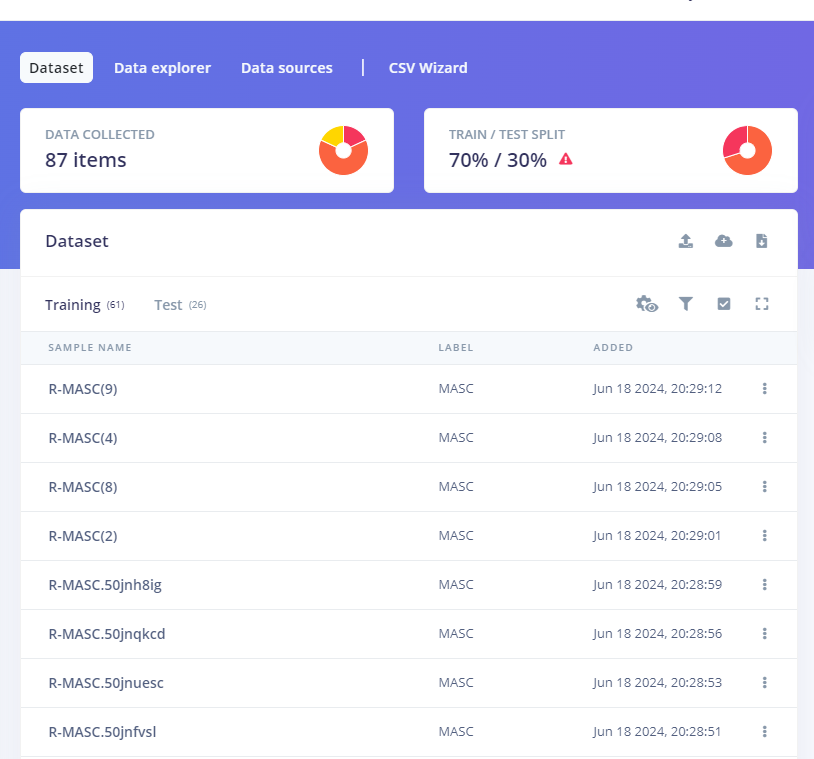
\includegraphics[width=130mm]{./Figuras/Desarrollo_Analisis/ADQUISION_DE_DATOS}
\caption{Bloque de adquisición de datos.} 
\label{fig:data1}
\end{figure}

\subsubsection{Bloque de pre-procesamiento} 
Seguidamente se entra a la etapa de pre-procesamiento de los datos, en una primera etapa se seleccionan características importantes como el ajuste a las dimensiones de las imágenes con las que se entrenará el modelo. En este caso se seleccionó 68x68 como las dimensiones óptimas tomando en consideración el uso de memoria adecuado para la tarjeta.
\begin{figure}[H]
\centering
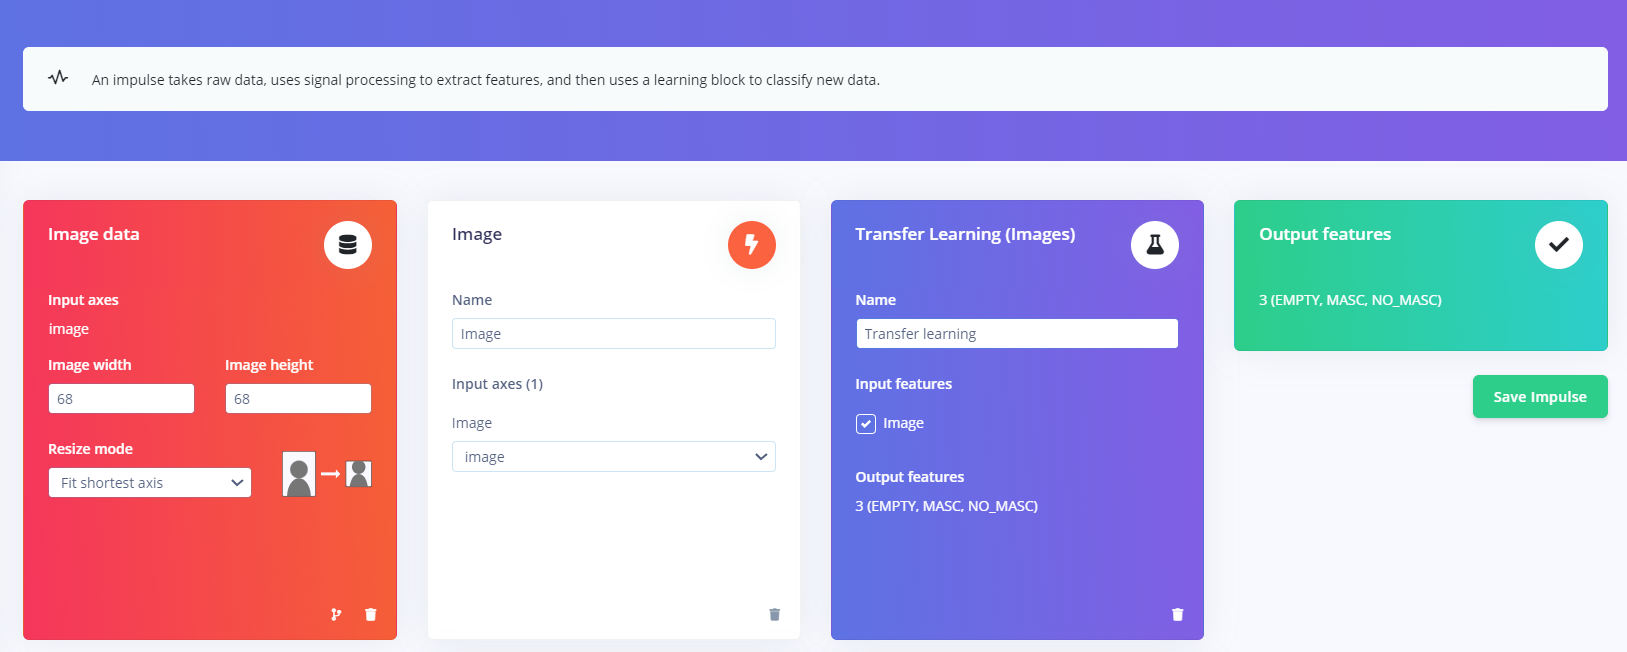
\includegraphics[width=150mm]{./Figuras/Desarrollo_Analisis/prepro1}
\caption{Bloque de adquisición de datos.} 
\label{fig:prepro1}
\end{figure}

Luego en la sección de image se pueden escoger parámetros como el tipo de color de las imágenes (RGB o Gray scale).
\begin{figure}[H]
\centering
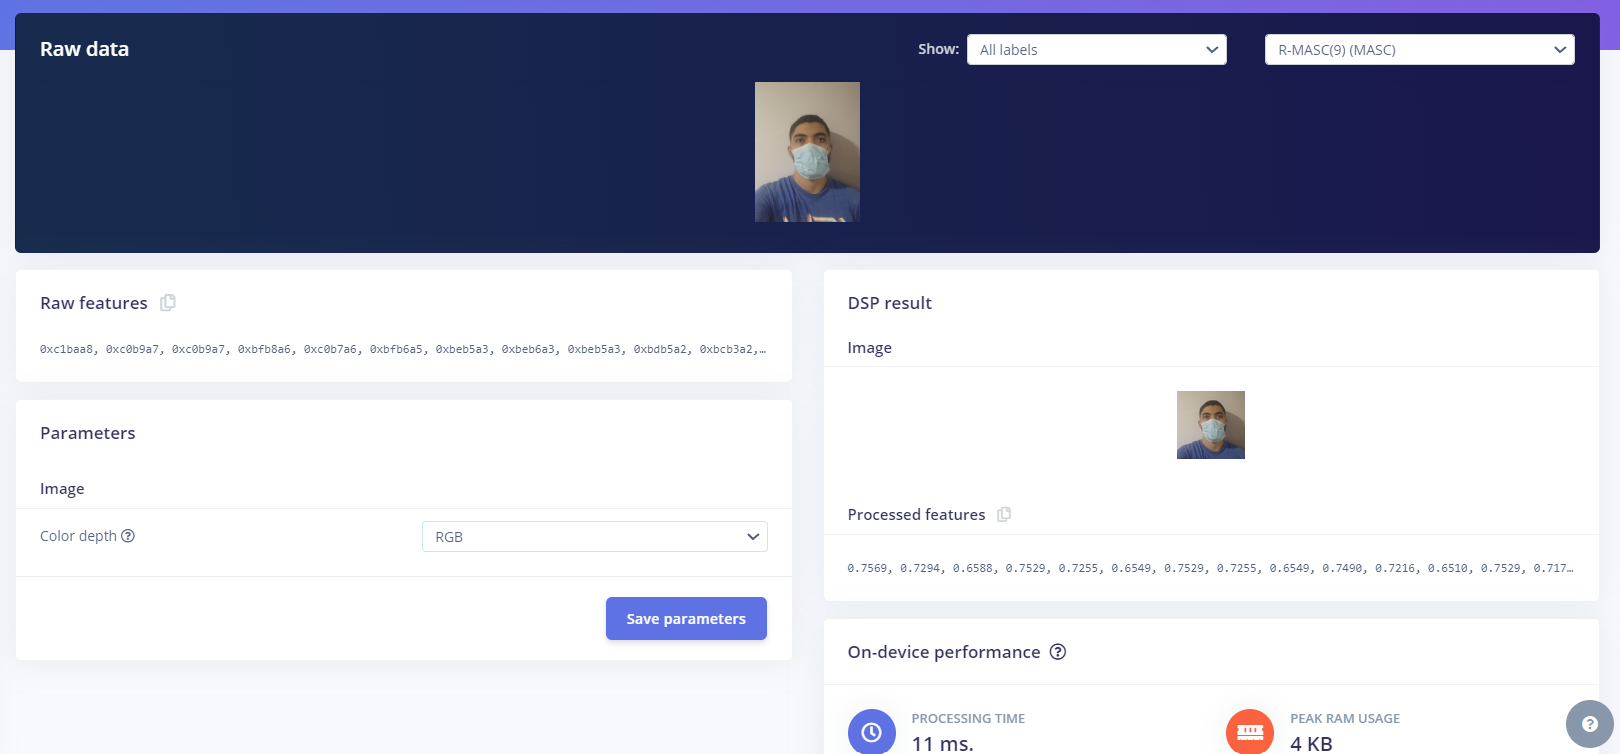
\includegraphics[width=150mm]{./Figuras/Desarrollo_Analisis/prepro2}
\caption{Bloque de adquisición de datos.} 
\label{fig:prepro2}
\end{figure}
\subsubsection{Selección de parámetros para el \textit{Transfer learning} del modelo}

En la Figura \ref{fig:PNN}, puede consultarse la selección de los parámetros utilizados para el entrenamiento del modelo en Edge Impulse:

\begin{figure}[H]
\centering
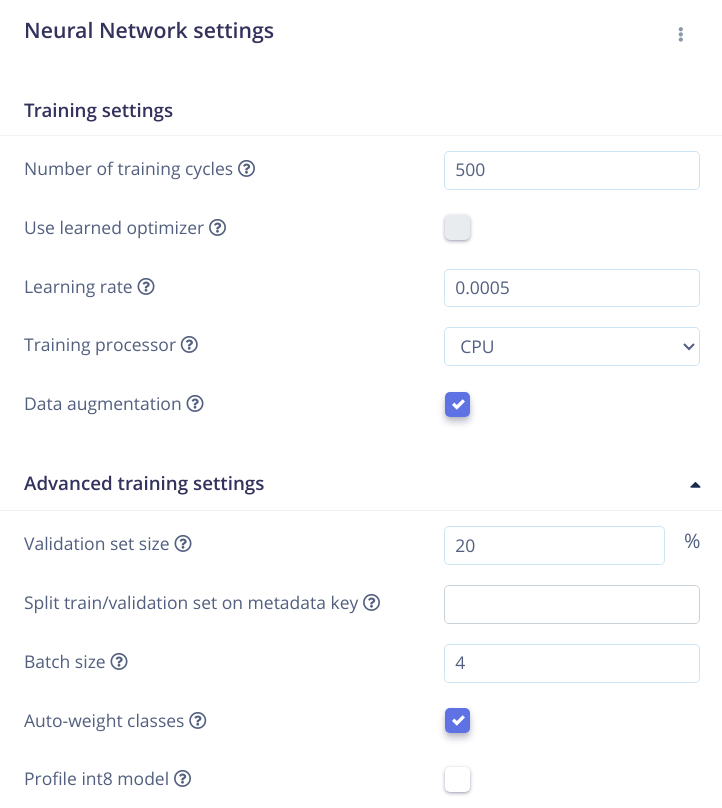
\includegraphics[width=120mm]{./Figuras/Desarrollo_Analisis/PNN}
\caption{Ajuste de los parámetros utilizados para ajustar el modelo en Edge Impulse.} 
\label{fig:PNN}
\end{figure}

A continuación se detalla de manera selección el porqué de la selección de este parámetro: 

\begin{itemize}
    \item \textit{\textbf{Number of training cycles}}: se seleccionó un valor grande (cercano al límite superior permitido por el plan gratuito de la plataforma) para asegurarse de que hubiera un buen margen para obtener una presición alta. 

    \item \textit{\textbf{Learning rate}}: se tomó un valor muy bajo para evitar un sobre-ajuste muy rápido del modelo.

    \item \textit{\textbf{Data augmentation}}: se habilitó, ya que permite ejecutar más ciclos de entrenamiento, aumentando la precisión. 

    \item \textit{\textbf{Validation set size}}: se toma la recomendación de la plataforma de utlizar un 20\% de conjunto de datos para validación. 

    \item \textit{\textbf{Batch size}}: se tomó un valor pequeño para permitir permite actualizaciones más frecuentes de los parámetros durante el entrenamiento, lo que ayuda a la convergencia del modelo y evita el sobreajuste de este.

    \item \textit{\textbf{Auto-weight classes}}: se habilitó, ya que no de todas las clase se tenía la misma cantidad de datos. 
\end{itemize}

Por otro lado, fue necesario seleccionar la arquitectura de la red neuronal, en la Figura \ref{fig:ANN}: 

\begin{figure}[H]
\centering
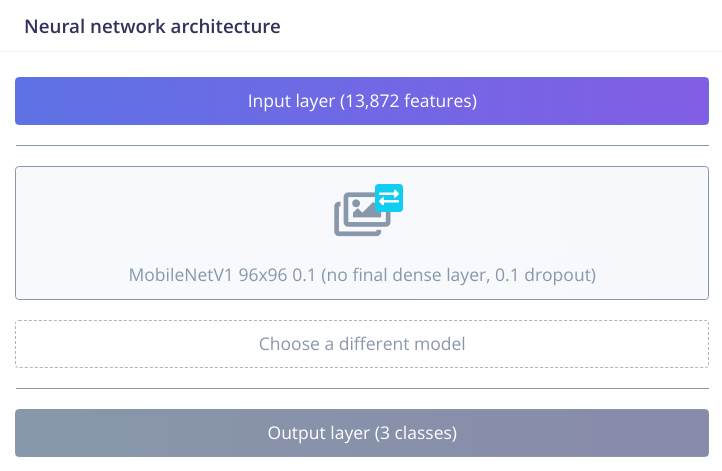
\includegraphics[width=120mm]{./Figuras/Desarrollo_Analisis/ANN}
\caption{Arquitectura seleccionada para entrenar el modelo en Edge Impulse.} 
\label{fig:ANN}
\end{figure}

Como puede verse en la Figura \ref{fig:ANN}, la arquitectura seleccionada fue la MobileNetV1 96x96 0.1, la cual utiliza aproximadamente 53.2 KB de RAM y 101 KB de ROM, utilizando las configuraciones por defecto y optimizaciones. Esta trabaja mejor con \textit{inputs} de 96x96 píxeles y soporta tanto la escala de grises como RGB. Se seleccionó esta, ya que es la utilizaba la menor cantidad de RAM y ROM, permitiendo cargar el modelo sin problemas al Arduino Nano 33 BLE. 

\subsection{Análisis de los resultados}
 A continuación se mostrarán los resultados para cada una de las funcionalidades solicitadas por el enunciado: 

\subsection{Rendimiento del entrenamiento del modelo}
En la Figura \ref{fig:RM}, puede observarse el rendimiento del entrenamiento del modelo, utilizando los datos cargados y los parámetros y arquitectura seleccionados: 

\begin{figure}[H]
\centering
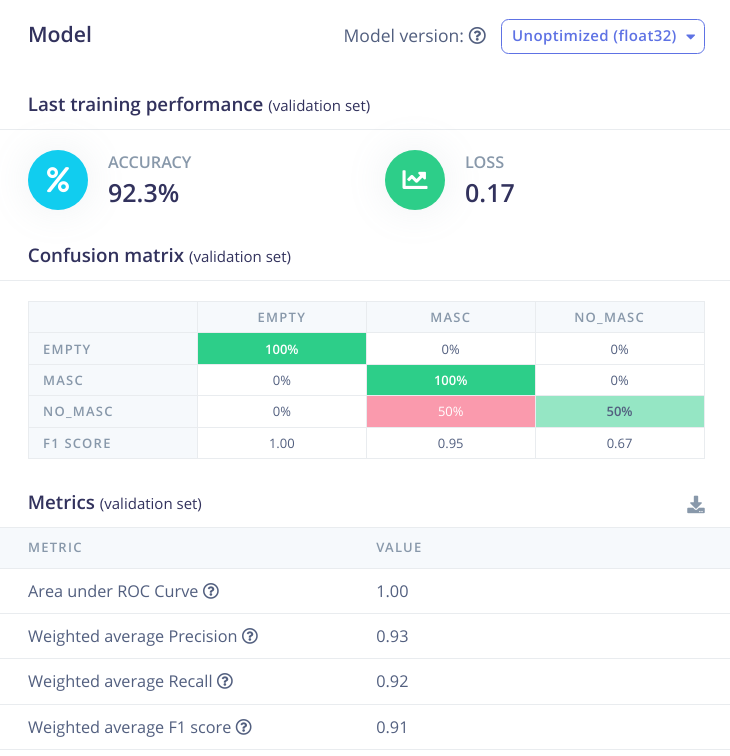
\includegraphics[width=120mm]{./Figuras/Desarrollo_Analisis/RM}
\caption{Rendimiento del entrenamiento del modelo tras el entrenamiento bajo las condiciones ya mencionadas.} 
\label{fig:RM}
\end{figure}

Como puede verse en la Figura \ref{fig:RM}, se tiene una precisión bastante alta del 92.3\%, lo que indica que al menos utilizando el porcentaje de validación indicado, el modelo se comporta bastante bien. Además se puede observar que la pérdida del modelo es bastante baja. 

\subsection{Rendimiento de la comprobación del modelo}
En la Figura \ref{fig:TM}, puede observarse el rendimiento de la comprobación del modelo tras ser entrenado y utilizando para esta los datos apartados para este propósito: 

\begin{figure}[H]
\centering
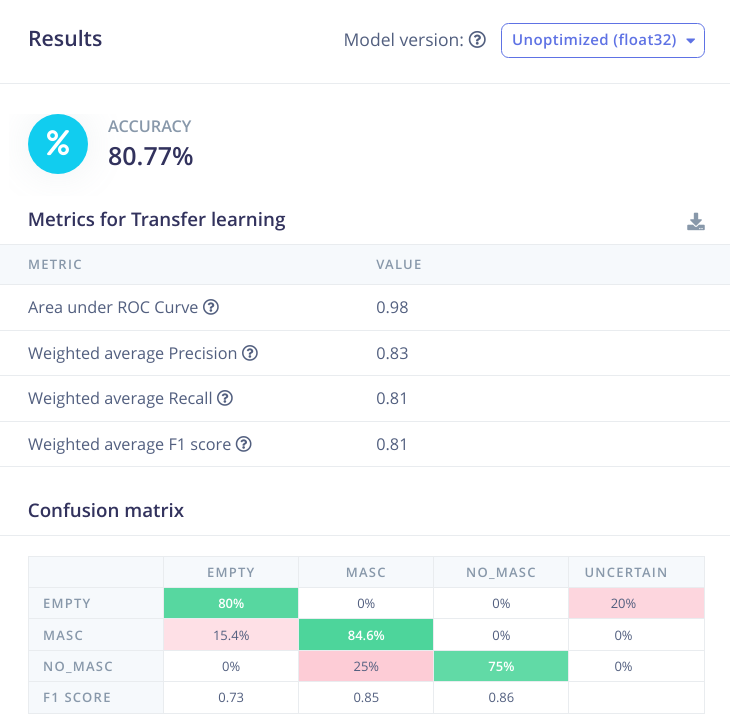
\includegraphics[width=120mm]{./Figuras/Desarrollo_Analisis/TM}
\caption{Rendimiento de la comprobación del modelo bajo las condiciones ya mencionadas.} 
\label{fig:TM}
\end{figure}

Como puede verse en la Figura \ref{fig:TM}, la comprobación tiene una precisión bastante alta del 80.77\%. Lo que indica que el modelo se comporta lo suficientemente bien para efectuar una identificación adecuada de un espacio vacío, una persona sin mascarilla y una con mascarilla. 

\subsection{Despliegue de información en la línea de comandos}
Una vez que el modelo es compilado y cargado en el microcontrolador, puede utilizarse la opción ``Serial Monitor'' del Arduino IDE para observaren en la línea de comandos los datos escritos en el puerto serial sobre el porcentaje de identificación según sea el caso.  En la Figura \ref{fig:SM} puede observarse un ejemplo de esto:

\begin{figure}[H]
\centering
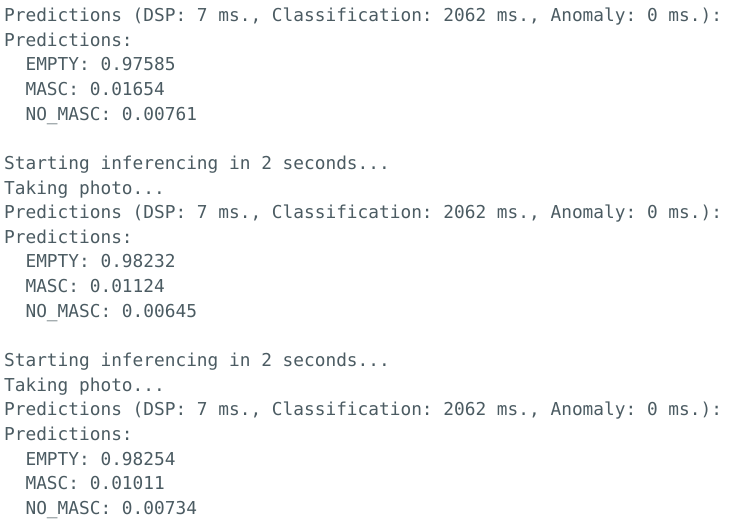
\includegraphics[width=130mm]{./Figuras/Desarrollo_Analisis/SM}
\caption{Impresión del porcentaje de identificación según sea el caso en el puerto serial.} 
\label{fig:SM}
\end{figure}

Como puede verse en la Figura \ref{fig:SM}, pueden observase las tres clases definidas para el modelo de identificación (EMPTY, MASC y NO\_MASC) y al lado el porcentaje asignado por este para cada caso. En el momento en el que se tomó esta captura, la cámara apuntaba hacia el techo de una habitación, es por esto que el porcentaje identificación de EMPTY es mayor que las otras dos clases.

\subsection{Identificación de clases y notificación con el LED RGB}
Para demostrar el funcionamiento del modelo de identificación es correcta y que la notificación de esta a través del LED RGB, puede consultarse en el siguiente video: \url{https://youtu.be/gyIAK8Mi2a0}. En este pueden observarse tres estados: 

\begin{enumerate}
    \item Al inicio del video puede observarse como mientras la cámara apunta hacia el vacío, el color azul es el que se mantiene en el LED RGB, indicando que la clase identificada es EMPTY. 
    
    \item Una vez que la cámara es apuntada a la cara de una persona sin mascarilla, el LED RGB cambia a rojo, indicando que la clase identificada es NO\_MASC.
    
    \item Al final del video, puede verse como al apuntarse la cámara a la cada de una persona con mascarilla, el LED RGB cambia a verde, indicando que la clase identificada es MASC.
\end{enumerate}

Estos tres estados confirman la identificación adecuada de las tres clases y especialmente la identificación de una persona con mascarilla y lo notifica cambiando el color del LED RGB, por lo que se cumple de manera exitosa con lo solicitado en el enunciado del laboratorio.  